This chapter discusses some of the functionality that was implemented for Certidude in Gitlab, the chosen CI/CD solution. Preparatory work included the needed migration from Certidude's publicly hosted git repository on Github to the (so far) private Gitlab instance that was setup during the analysis phase described in Chapter \ref{chapter:analysis}. 

Section \ref{sec:pylint-pytest-bandit-sonarqube} describes the setup of an initial pipeline for Certidude where code quality tools are integrated to analyze Certidude's code base. See Chapter \ref{chapter:concepts} for more details on these tools. Section \ref{vbox-cert} describes how new build environments can be provisioned using the Gitlab VirtualBox runner. Section \ref{openwrt} describes an implemented step in the pipeline to compile OpenWrt images. This chapter concludes with section \ref{future-work}, where a list was compiled of features and tasks that would expand and improve upon this work.

Appendices \hyperref[chapter:appendix-certidude-pipeline]{6}, \hyperref[chapter:appendix-sonar]{7}, \hyperref[chapter:appendix-vbox]{8} and \hyperref[chapter:appendix-openwrt]{9} contain produced configuration files, pipeline definition files and used instructions to produce a VirtualBox based build agent which can launch a VM and integrate with Gitlab CI.

\section{Pylint, Pytest, Bandit and SonarQube} \label{sec:pylint-pytest-bandit-sonarqube}
A basic pipeline was created with \textit{build, test and scan} stages for Certidude and the associated YAML file was included into the repository so as to be able to trigger it. See Appendix \hyperref[chapter:appendix-certidude-pipeline]{6} for the full declaration of this pipeline. Its \textit{build} phase contains one task: "\textit{sonar\_docker}". It starts a docker image containing SonarQube by first pulling it from the docker repository which is integrated into Gitlab and then issuing the command to initiate its main process. This sets up the web service that will later take in and visualize test and scan reports. 

The inbuilt docker registry of Gitlab is hosted by default through port 5001. The following commands show how the docker image provided by SonarQube was pulled from their public repository, tagged and pushed to Gitlab's private one. This was mainly done to help speed up the build process.

\pagebreak

\begin{figure}[H]
\centering
\begin{lstlisting}[frame=single, basicstyle=\small, linewidth=\textwidth]
user@host:~# docker login -u <username> -p <password> \\ 
                                        <ip/host>:5001
user@host:~# docker pull sonarqube
user@host:~# docker tag sonarqube:latest \\
                    <ip/host>:5001/certidude/certidude:sonarqube
user@host:~# docker push <ip>:5001/certidude/certidude:sonarqube
\end{lstlisting}
\caption{\textit{Pushing a SonarQube image to the Docker registery in Gitlab.}}
\label{fig:gitlab-sonar-docker}
\end{figure}

The \textit{test} stage contains three tasks: "\textit{Pylint, Pytest and Bandit}". These three parallel tasks each produce report artifacts which are uploaded to Gitlab. They indicate which tests passed or failed, which lines of code were covered by those tests, conformity to coding standards and possible security issues encountered. These reports are produced in a structured format (e.g. JSON / XML) and which are later consumed by SonarQube. The "dependencies" section of a task in Gitlab's YAML syntax is needed to indicate what earlier produced artifacts will be downloaded into the working directory where the current task is being executed.

In the final \textit{scan} stage we can see one task "\textit{sonar\_scan}" which takes in all previously generated reports. It also installs SonarQube's active scanner utility and scans Certidude's code based on a profile of defined rules hosted on the previously started SonarQube instance. See Figure \ref{fig:sonarqube-profiles} for how the default Python profile was extended to include more rules. The utility needs a configuration file to interact with the main server which was included in Appendix \hyperref[chapter:appendix-sonar]{7}. After the scan is complete the utility uploads its results and all the previously generated reports to the main SonarQube server for visualization and analysis. Figure \ref{fig:sonarqube-result} shows part of Certidude's results visualized in SonarQube. Here all previously gathered reports and information is condensed into one place. The following points describe parts of the image.

\begin{enumerate}
    \item Name of the project and file currently under review. The project was named \textit{Certidude} and \textit{cli.py} is currently being analyzed.
    \item A vulnerability rule was triggered and this indicates the offending line. A variable command is executed in a subshell which could indicate a possibility of command injection if the variable is manipulable.
    \item Source of this triggered rule, in this case the report generated by \textit{Bandit}. It also shows the inbuilt ticketing system and classification of the triggered rule.
    \item Shows the date and commit hash identifying when this piece of the code was contributed.
    \item Red and green annotations placed next to each line are based on the provided code coverage reports and indicate whether that line was executed during the tests. 
\end{enumerate}

\begin{figure}[!htb]
    \centering
    \begin{minipage}{.5\textwidth}
        \centering
        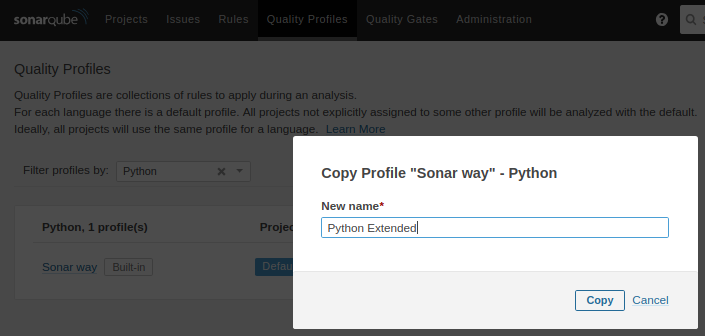
\includegraphics[width=.95\linewidth]{figures/screenshots/sonar-profile.png}
    \end{minipage}%
    \begin{minipage}{0.5\textwidth}
        \centering
        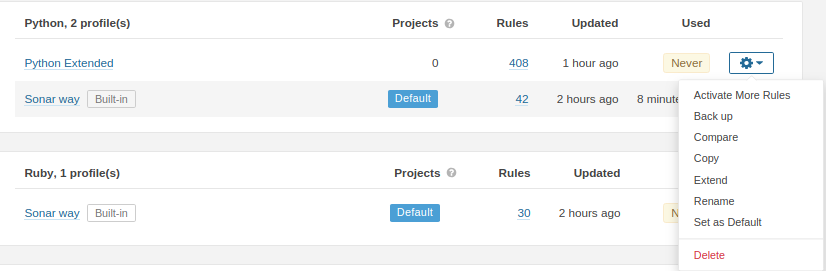
\includegraphics[width=.95\linewidth]{figures/screenshots/sonar-python-profile.png}
    \end{minipage}
    \captionof{figure}{\textit{SonarQube: Extending the default Python security profile and its rulebase.}}
    \label{fig:sonarqube-profiles}
\end{figure}

\begin{figure}[!htb]
    \centering
    \begin{minipage}{\textwidth}
    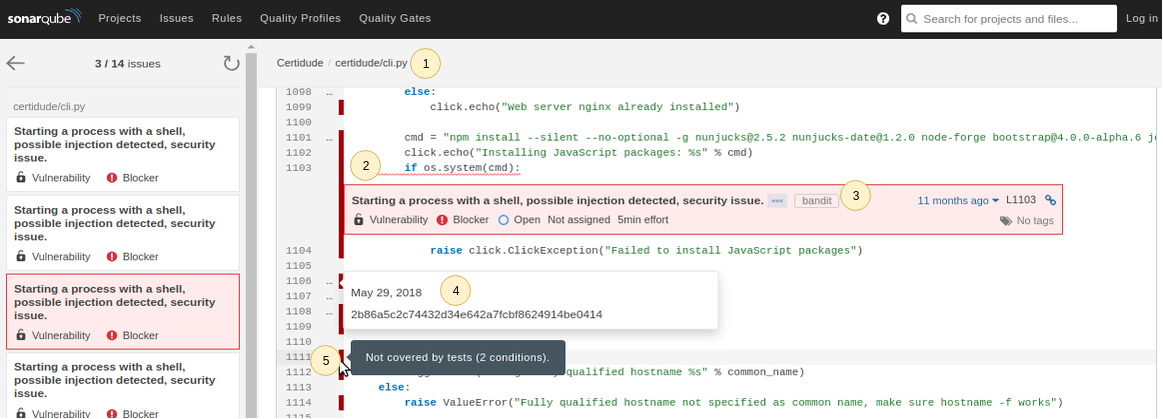
\includegraphics[width=1\linewidth]{figures/screenshots/sonarqube-analysis3.png}
    \end{minipage}
    \captionof{figure}{\textit{SonarQube: Code analysis and visualizations.}}
    \label{fig:sonarqube-result}
\end{figure}

An interesting feature that can also be observed in this pipeline is inheritance of instructions between tasks. This aims to clean up the pipeline file by reuse of the same code block through references instead of duplicating code. In Figure \ref{fig:yaml-anchor} one can see a reference (\textit{\&install-deps}) being created for a hidden task (\textit{.python-install-dependencies}). One can hide a task from being run by prepending a dot to the name of the task and will prevent it from being executed. In inheriting tasks (e.g. \textit{Pylint}) this "pointer" to the task is "de-referenced" (\textit{*install-deps}) which inserts the code block belonging to the task in its place.

\begin{figure}[H]
\centering
\begin{lstlisting}[frame=single, basicstyle=\small, linewidth=\textwidth]
.python-install-dependencies: &install-deps |-
  sudo apt-get update -qy
  ...
  
pylint:
  stage: test
  before_script:
    - *install-deps
  ...
\end{lstlisting}
\caption{\textit{Inheritance through YAML anchors in Gitlab configuration files.}}
\label{fig:yaml-anchor}
\end{figure}

\section{VirtualBox}\label{vbox-cert}
So far only a native shell build agent has been used, which means the agent fetches instructions from the CI/CD server and tries to execute any shell commands as the user that runs the agent. This is done in a temporary working directory created for that task. For Gitlab the default \textit{gitlab-runner} user is used which gets created when the agent is installed.\cite{gitlab-runner} In Gitlab terminology a build agent is also referred to as a runner and how this runner executes its fetched instructions is referred to as "\textit{executor}". A runner needs to be registered to the main CI/CD server, where it authenticates and indicates its executor type (e.g. Shell or VirtualBox), configuration options (e.g. name of VM or snapshot) and any associated tags. Multiple runners can be registered on the same machine using different executors. Tags are a way for the main CI/CD server to designate tasks to specific runners and/or executors. 

Best practice would be to have access to reusable virtual environments though and Gitlab integrates well with Docker and VirtualBox to provide these. While docker containers were previously used through shell commands (and have a nicer YAML syntax as well for docker executor), preference sometimes goes towards having full-fledged virtual machines available. This is also the case for Certidude, its tests and some of the components it needs to interact with.

Gitlab-runner was installed on the author's personal laptop which was connected over a VPN to the Gitlab CI instance.\cite{gitlab-runner} VirtualBox was installed, an Ubuntu 16.04 VM was created and OpenSSH server installed within, key based access was setup and the runner was registered to the Gitlab CI instance as a VirtualBox executor, pointing to the created VM. In addition the runner was also setup in the VM itself so as to allow for artifact uploads back to the CI/CD server. Several guides were used to do all this, including one provided by Gitlab.\cite{vbox-cli, vbox-oracle, gitlab-runner} All the steps that were performed are included in Appendix \hyperref[chapter:appendix-vbox]{8}. Using the executor is done transparently by simply including the registered tag for that executor in the defined pipeline task.

Figure \ref{fig:gitlab-runner-conf} shows the subsequent configuration file that was created in "\textit{/etc/gitlab-runner/config.toml}"

\pagebreak


\begin{figure}[H]
\centering
\begin{lstlisting}[frame=single, basicstyle=\small, linewidth=\textwidth]
[[runners]]
  name = "VirtualBox Runner"
  url = "https://<address/ip>/"
  token = "some-secret-shared-between-the-runner-and-server"
  executor = "virtualbox"
  [runners.custom_build_dir]
  [runners.ssh]
    user = "username"
    password = "password"
    identity_file = "/home/user/.ssh/id_rsa_vbox_runner"
  [runners.virtualbox]
    base_name = "Ubuntu-1604"
    disable_snapshots = false
  [runners.cache]
    [runners.cache.s3]
    [runners.cache.gcs]
\end{lstlisting}
\caption{\textit{Gitlab Virtualbox-Runner configuration file.}}
\label{fig:gitlab-runner-conf}
\end{figure}

\section{OpenWrt}\label{openwrt}

One request from supervisor and main developer of Certidude, \supervisor, was to have an OpenWrt image compilation step. OpenWrt is a Linux OS targeting embedded devices like routers.\cite{openwrt} The reason for this desire is to assist IOT (Internet Of Things) devices that don't support modern cryptographic libraries to still communicate over secure channels with the outside world. This would be done by transparently encrypting traffic through a VPN by the custom firmware image created which would be flashed on a small router placed between the device and the outside world. In this scenario Certidude would be the tool to help orchestrate and manage any certificate signing and validation. 

Appendix \hyperref[chapter:appendix-openwrt]{9} shows the created pipeline step to produce a custom OpenWrt image. The actual image customization has been left out, but would be integrated in the script-part of the \textit{build\_image} job.\cite{openwrt-build} This step extends Continuous Integration into Continuous Delivery for Certidude by producing a production ready router image. It shows how artifact creation and possible deployment steps are a natural extension of the CI development practice. 

\pagebreak

\section{Future Work} \label{future-work}
Future work involves dissecting, correcting and expanding the current test suite of Certidude which is not passing at the moment of this writing. Some of the current tests assume behavior no longer present in the code base while other code has been altered enough to break the tests (e.g. structure of API calls). The following list contains some concrete suggestions for future improvement.

\begin{itemize}
    \item The current setup of Gitlab and SonarQube are private but could instead be moved to a dedicated public facing address. SSL (Secure Sockets Layer) / TLS (Transport Layer Security) certificates need to be setup and SonarQube needs to be properly installed alongside some supporting database solution.
    \item The current test suite contains a complex sequence of services being provisioned to test integration with Certidude. These services include a Samba DC, OpenVPN / StrongSwan clients and gateways. The provisioning of these services lend themselves perfectly for both parallelization as well as virtualization. This would mean launching various containers and virtual machines at the same time providing these services. This is now possible.
    \item More integration tests for FreeBSD, Juniper, Cisco and Windows. This would involve expanding on the VM runner integration of Gitlab CI. Perhaps a GNS3 VM could potentially be used to simulate complex network scenarios with Cisco or using Junos OS based vMX virtual router. There is also Docker for Windows available which was not explored in this work.
    \item More CD pipeline steps to build and deploy code. This could include integration with a configuration management system like Chef, Puppet or Ansible as well as package creation (e.g. pip).
    \item Expand the integration test suite by including Selenium. This would require a build step where Certidude gets fully built and run.  
    \item Expand on the security test suite by putting tools like OWASP ZAP between the integration tests written with Selenium and the Certidude instance or use clair to perform container vulnerability scans. At the moment of this writing there is an attempt being made to properly containerize Certidude which would make this last addition more relevant.
\end{itemize}








\pagebreak
\pagebreak



\iffalse % Starts dummy text

\begin{itemize}
    \item Deconstruct Certidude here a bit
    \item Deconstruct its tests; this is quite hard at the moment since they are not up-to-date
    \item 
\end{itemize}


* Dockerfiles for OpenVPN / StrongSwan / WireGuard
Alpine vs. Centos vs. Ubuntu..?


% This is might be because of defaul EE edition, no bronze/gold/ultimate.. this could be requested? 
% I suspect it just needs formatting
* pylint reports can be generated in json format, but gitlabci expects these to be in predefined format 
\url{https://docs.gitlab.com/ee/user/project/merge_requests/code_quality.html}
\url{https://docs.gitlab.com/ee/user/project/pipelines/job_artifacts.html}
\url{https://docs.pylint.org/en/1.6.0/output.html}
\url{https://realpython.com/python-json/}
Upload of artifacts fails using artififacts:reports:junit / codequality etc. Normal upload works. 
Maybe try to convert pylint report into right format anyways? Also for bandit?
pylint --output-format=json example/ >> pylint1.json 

* Describe sonarube install? \url{https://docs.sonarqube.org/latest/setup/get-started-2-minutes/}
  See for scanner install: \url{https://docs.sonarqube.org/display/SCAN/Analyzing+with+SonarQube+Scanner}
  Then see about sonarpython \url{https://docs.sonarqube.org/display/PLUG/SonarPython}
 
 - docker pull sonarqube:latest
   docker run -d --name sonarqube -p 9000:9000 sonarqube
 - Download / Install:  \url{https://binaries.sonarsource.com/Distribution/sonar-scanner-cli/sonar-scanner-cli-3.3.0.1492-linux.zip}
 
 - Setting the sonar.python.coverage.reportPaths variable in home directory config file to point to coverage file..
 - login as admin/admin -> administration -> marketplace -> python this way you can also install the sonarpyhton plugin
 - login as admin/admin -> Quality Profiles -> should show the python one, but a lot of rules are deactivated
   -> bulk change and activate all (non-depricated) rules -> back to quality profiles and set new one as default..
 - \url{https://docs.sonarqube.org/latest/analysis/analysis-parameters/}
 - atm link back to source code files is not present in junit test reports, so it will only show that there are x failing tests..
   \url{https://stackoverflow.com/questions/29117785/no-drilldown-from-sonarqube-unit-test-success-widget}
   
 - set .profile to include solar-scanner/bin as part of PATH for gitlab-runner user..
 
\fi % Ends dummy text